\documentclass{article}
\usepackage{microtype,graphicx,booktabs,hyperref}
\usepackage{icml2027}
\usepackage{amsmath,amssymb,amsthm,placeins}
\newtheorem{theorem}{Theorem}
\newtheorem{proposition}[theorem]{Proposition}
\newcommand{\gap}{\operatorname{gap}}
\newcommand{\opt}{\operatorname{OPT}}
\icmltitlerunning{When Is Immediate Refill Optimal for Parallel Voting?}
\begin{document}
\twocolumn[
\icmltitle{When Is Immediate Refill Optimal for Parallel Voting?}
\begin{icmlauthorlist}
\icmlauthor{Anonymous Authors}{anon}
\end{icmlauthorlist}
\icmlaffiliation{anon}{Anonymous Institution}
\icmlcorrespondingauthor{Anonymous Author}{anonymous@example.org}
\icmlkeywords{test-time computation, adaptive inference, scheduling, parallel voting}
\vskip 0.3in
]
\printAffiliationsAndNotice{}
\begin{abstract}
A reasoning service with a free generation slot must decide whether to start the next sample. We study ordered, irrevocable starts and a per-question allowance beyond the serial vote. Fix the slot count and a common width-dependent decode clock. At zero allowance, immediate refill is optimal across all panel sizes, launch quotas, positive path lengths and votes if and only if step cost is discretely concave. Its least concave majorant gives the exact worst-case time ratio over that class. On an A800, calibration predicted that deferring one of three prescribed Qwen2.5-1.5B requests would save 3.13\%. Twelve paired measurements gave a median whole-panel saving of 2.46\%. On three-path prefixes of 200 archived GSM8K questions, foreknowledge of the lengths could save at most 0.364\% on average by choosing between the same two actions under this clock. Allowing one extra launch raises a different question about out-of-order votes. On the 200 questions, fully indexed admission saved 8.71\% of modeled time over a gate using only contiguous-prefix votes. Against a gate retaining completed positions and all vote counts, it saved 0.67\%. Retaining the vote-to-position pairs in the contiguous prefix as well narrowed the gain to 0.30\%.
\end{abstract}

\section{Introduction}
Suppose a reasoning service may commission sixteen solutions to a math question and return their plurality vote. It has four generation slots. Long solutions and short solutions run together, so the fourth path to start can finish before the first. When a slot opens, should the service use this newly arrived vote to start another sample? Should it sometimes leave the slot empty so that the requests already in progress finish sooner?

These questions require different comparisons. For admission, each scheduler fills every slot its information permits. We vary which returned votes it can count and which votes it can associate with their positions. For timing, both schedulers have all available information and differ only in whether to delay a legal start.

A request quota makes the distinction consequential. Consider a service promising to launch at most one request more than the number its serial counterpart would have needed on the same ordered votes. If the first nine votes would settle a question, the tenth launch is permissible and the eleventh spends a request beyond the allowance. The service learns which votes suffice only after they return. An absolute cap of fourteen starts can apply simultaneously. This contract controls irreversible starts for each question. A provider concerned only with average token cost or with outstanding cancellations can legitimately choose a different policy.

We first ask when a service can fill every admissible slot with a pathwise optimality guarantee. With zero extra starts and equal votes, every schedule completes the same paths. Greedy refill concentrates their work in intervals of high occupancy. We prove that this concentration is maximal at every occupancy threshold, for arbitrarily many slots. It gives an exact test on the width-dependent step costs for immediate refill to minimize decision time on all panels. The test also gives a quantitative approximation guarantee for a measured clock that departs from concavity.

Allowing a single extra start can change which paths finish and how much work is lost at cancellation. We lower-bound the decision time attainable in this case by charging for the work that any putative final voting certificate already requires. We then measure how much time is available to recover by using out-of-order votes or by delaying a legal start. We compare two levels of admission information short of retaining every vote's index. A small change in the information available to the baseline accounts for most of the larger replay gain. Device experiments distinguish changes in dispatch from changes in wall time.

\section{Voting and admission}\label{sec:front}
Fix \(N\) indexed paths of positive work \(w_i\) and terminal votes \(v_i\). A vote is a discrete label or an abstention. For a set \(S\) of completed indexed observations, \(\gap(S)\) is the largest label count minus the second largest. Absent labels have count zero. A strict lock occurs when
\[
                       \gap(S)>N-|S|.
\]
Even if all unknown votes favored the runner-up, the leader would still win. The service returns immediately at a strict lock. Exhaustion returns the plurality under a common tie rule. The absolute quota is an integer \(1\le Q\le N\). When \(Q<N\), the service drains its \(Q\) starts if necessary and marks the result uncertified when it cannot establish a full-panel winner. Abstentions count as completed work. Agreement with the full vote and numerical answer accuracy are distinct outcomes.

Let \(K(v)\) denote the first decisive serial prefix, with \(K=N\) on exhaustion. A service with \(P\) slots must ensure \(J\le K(v)+B\), where \(J\) counts all starts, including subsequent cancellations. The guarantee ranges over every joint assignment of the unseen votes compatible with the observed votes. Elapsed service time imposes no further restriction on those assignments. Starts occur in index order, and each path occupies a slot until completion or return.

On a nonterminal history, let \(S_t\) be the observed votes among the first \(t\) indices. Define
\begin{align}
 M(S)&=\min\bigl(\{t<N:\gap(S_t)+t-|S_t|>N-t\}\nonumber\\[-2pt]
     &\hspace{3.65cm}\cup\{N\}\bigr),\label{eq:m}\\
 F(S)&=\min\{Q,\ |S|+P,\ M(S)+B\}.\label{eq:f}
\end{align}
At prefix \(t\), assigning all its missing votes to a current leader maximizes the margin and attains the left side of the inequality in \eqref{eq:m}. Thus \(M\) is the earliest serial stop among compatible assignments. Starting past \(M+B\) violates the promise on an attaining assignment. Hence \(F\) is the exact safe cumulative launch count. It can be computed by a scan maintaining the two largest label counts. More observations restrict the compatible assignments, so \(F\) cannot decrease.

The \emph{indexed} policy \(G\) immediately fills to \(F\). The \emph{buffered} policy uses only the longest contiguous completed prefix to compute \(M\). Both use the actual number of completions for slot capacity, stop using all returned votes, and charge the same starts. To see the difference, take \(N=Q=5\), \(P=3\) and \(B=1\). Paths 2 and 3 have returned A and B while paths 1 and 4 run. The first three votes cannot lead by more than one, too little to cover the last two votes. Thus \(M=4\) and \(G\) may start path 5. The contiguous prefix is empty. Viewed through it, the first three votes could all be A, giving \(M=3\). The buffered gate leaves a slot free.

\section{The cost of an admissible start}
\paragraph{A common clock.}
At width \(k\), all active paths process work at rate \(1/c_k\) with \(c_k>0\). One unit of \emph{virtual time} advances every active path by one unit of work, and costs \(c_k\) units of elapsed time. Let \(V_A\) and \(T_A\) denote the virtual and physical decision times of a policy \(A\). Let \(d_k\) be its virtual time at width \(k\). Then \(V_A=\sum_k d_k\), generated work is \(\sum_k k d_k\), and \(T_A=\sum_k c_kd_k\). Empty-system delays can be removed. Initial work, terminal votes and admissible actions are shared between policies.

By the virtual time a safe comparator \(A\) starts path \(i\), \(G\) has either started \(i\) or already returned. To see this, induct on launches while \(G\) is running. Each earlier path takes \(w_j\) after launch, so every observation used by \(A\) has also reached \(G\). Its frontier therefore permits at least the same cumulative starts. At \(A\)'s decision, an unreturned \(G\) would likewise have observed its lock or completed its quota. Hence \(V_G\le V_A\) and \(T_A\ge V_G\min_k c_k\). We sharpen this time bound using occupancy at zero allowance and certificate work at positive allowance.

\subsection{Universal optimality at zero allowance}
The zero-overrun contract forces every policy to complete the same prefix of length $\min(K,Q)$ and consume the same work $W_*$ (Appendix~\ref{app:zero}). Let $h_A(t)$ count the active paths in virtual time, with zero after the decision. Greedy's occupancy decreases as votes return. The stronger fact is that even the busiest intervals of a comparator cannot collectively process more work than an equally long initial interval of greedy.

\begin{theorem}[Immediate refill at any slot count]\label{th:occupancy}
Fix $P\ge1$ and positive width costs $c_1,\ldots,c_P$, with $c_0=0$. Let $\mathcal I$ be the class of zero-allowance instances with arbitrary panel size $N\ge1$, quota $1\le Q\le N$, positive path lengths and equal-weight terminal votes. Greedy minimizes wall time on every $I\in\mathcal I$ if and only if
\[
      2c_j\ge c_{j-1}+c_{j+1},\qquad 1\le j<P .
\]
Let $\widehat c$ be the least concave majorant on $0,\ldots,P$. Writing $T_{\rm opt}$ for the infimum over legal schedules on the given instance, we have
\[
  \sup_{I\in\mathcal I}\frac{T_G(I)}{T_{\rm opt}(I)}
            = \max_{1\le k\le P}\frac{\widehat c_k}{c_k} .
\]
For any admissible schedule $A$ and union $E$ of intervals of its virtual timeline,
\begin{equation}\label{eq:major}
       \int_E h_A(t)\,dt\ \le\ \int_0^{|E|} h_G(t)\,dt .
\end{equation}
\end{theorem}
The proof shortens a competitor's timeline outside $E$, preserving the order of all observations and starts. Each job now requires weakly less work. On this shortened input greedy finishes earlier, but its width at any given time can only fall because earlier completions tighten the remaining allowance for active paths. This comparison gives \eqref{eq:major}. Applying it to $E=\{h_A>j\}$ shows that greedy maximizes the integrated excess above every width $j$. Discrete concavity makes each such excess reduce the total price for a fixed amount of work. For necessity, a panel of long and short paths realizes the comparison $c_{j-1}+c_{j+1}$ against $2c_j$. Appendix~\ref{app:major} proves these steps, including arbitrary continuous launch delays. Earliest completion of each job alone does not imply \eqref{eq:major}. On a four-job precedence graph greedy finishes every job by the corresponding competitor's finish time in virtual time, yet costs $4$ against $3.75$ on a concave clock (Appendix~\ref{app:precedence}).

For $P=3$ and prices $(10,11,13)$ the universal ratio is $23/22$. Four paths with works $(2,1,1,2)$, votes AAAB and $Q=3$ attain it. Greedy costs $13+10=23$, while starting two paths and replacing the first short finisher costs $2\times11=22$. Fixing $N=Q=3$ instead gives worst-case ratio one. Two initial votes could lock, so at most two paths may start before the first return. At most two then remain. The reachable prices $(0,10,11)$ are concave.

\paragraph{Imperfect concavity.} Put $\gamma=\max_{1\le k\le P}\widehat c_k/c_k$. Fix an execution of $A$ at prices $c$, with virtual occupancy durations $d_k$. Replaying its virtual launch times preserves the votes observed at each launch and hence its legality under $\widehat c$. Greedy also has the same virtual trajectory at both prices. Applying concave optimality to the replay gives
\[
 T_G(c)\le T_G(\widehat c)\le \sum_k\widehat c_k d_k
 \le \gamma \sum_k c_k d_k=\gamma T_A(c).
\]
For sharpness, take a chord of $\widehat c$ spanning a maximizing width $j$. A prefix of short agreeing votes sets the admissible width to the chord's upper endpoint. An ensuing set of opposite votes holds that limit fixed while greedy moves between the two endpoint widths and a competitor stays at $j$. As the prefix work vanishes the resulting time ratio converges to $\gamma$ (Appendix~\ref{app:sharp}).

\subsection{A lower bound from terminal certificates}\label{sec:lb}
For any possible set \(S\) of paths that have finished by the decision, path \(i\) has received at least
\begin{equation}
 a_i(S)=\min\{w_i,\ \max_{j\in S,\;j\ge i} w_j\},
 \label{eq:work}
\end{equation}
with an empty maximum equal to zero. Indeed, to finish \(j\) the service must advance it by \(w_j\) after launch. Every earlier indexed path has already started, and either receives this much work or has finished. For example, a certificate that requires the fourth path to return after 100 work units also obliges the service to spend up to 100 units on each of the first three. This charge can exceed the sum of the finished paths' lengths.

Let \(W_m(S)\) sum the \(m\) largest lower bounds \(a_i(S)\), and let \(W(S)=\sum_i a_i(S)\). Extend \(G\)'s virtual run past its first lock by retaining active paths and filling all available slots up to \(Q\). Write \(e_i\) for its completion times. Each provides an optimistic finish time for the corresponding path in a compliant schedule.

\begin{theorem}[Certificate work bound]\label{th:floor}
For each candidate \(S\), minimize \(\sum_{k=1}^P c_k d_k\) over \(d_k\ge0\) subject to
\begin{align}
 \sum_k d_k &\ge \max\{V_G,\max_{i\in S}e_i\}, \nonumber\\
 \sum_k\min(k,m)d_k &\ge W_m(S) \quad (1\le m<P), \label{eq:lp}\\
 \sum_k k d_k &\ge W(S). \nonumber
\end{align}
If the enumerated family contains every attainable terminal completed set, the minimum of these optima lower-bounds the physical decision time of every comparator that satisfies the public-history launch guarantees. The comparator may use foreknowledge of works and votes to select among its legal actions.
\end{theorem}
\begin{proof}
Before its lock the extended run inherits the virtual launch-time dominance of \(G\). Subsequently it faces only slot and quota limits. Whenever a comparator launches, the extended run has at least its observed completions and can accommodate the same cumulative launch count. Hence no job finished by the comparator can finish before \(e_i\). At width \(k\), any designated \(m\) paths can receive at most \(\min(k,m)\) combined work per virtual unit, and all paths receive \(k\) in total. Applying \eqref{eq:work} to the actual completed set proves feasibility of its occupancy vector. Minimizing over a superset preserves the lower bound.
\end{proof}

A feasible relaxation may combine service intervals that no single scheduler can realize. Its value supplies a ceiling \(1-\mathrm{LB}/T_G\) on potential fractional improvement over \(G\). Subsets are cheap to enumerate for \(Q=14\). They need either a strict certificate or full quota completion. If \(j\) finished, every earlier \(i\) with \(w_i\le w_j\) must also have finished. We discard masks failing this condition and masks whose most advanced completed path could not have been admitted. Dominated requirement vectors can also be dropped. At most four vectors remained on any of the 124 previously studied panels.

\paragraph{The cost of waiting.} One extra start permits a policy to postpone a short decisive vote behind an arbitrarily long running path, incurring unbounded relative delay. If postponements have total virtual duration $H$, the extra virtual delay is at most $H$. Appendix~\ref{app:timer} gives the sharp example and proof.

\section{Where does the time go?}\label{sec:exp}
\paragraph{Evaluation design.}
We fixed \(N=16,P=4,Q=14,B=1\) for the primary comparison. In fixed-trace replay, a path returns its archived vote at its recorded output length. A decision is certified when the observed margin beats every assignment of the remaining votes, including unlaunched paths beyond the absolute cap. Both admission gates thus agree on certification and output for fixed votes. A change in the set of co-runners can alter sampled tokens on a real engine. We consider controlled generation and natural generation separately.

We used three previously studied cohorts to audit the bound. AIME 2025 contains 30 problems, each with two disjoint panels, and AMC 2023 supplies 40 second-draw panels. Their unsteered paths come from Qwen3-4B-Base and the same public trajectory publisher. The OlympiadBench cohort \citep{he2024olympiadbench} contains 24 independently selected English integer-answer questions generated with DeepSeek-R1-Distill-Qwen-1.5B. We archived one full reference panel per question. The matched AIME comparison was retrospective. We also evaluated a new GSM8K split \citep{gsm8k}, freezing the comparison, question selection and primary clock before retrieving its trajectories.

For each question, we sum its policy times across its panels and compute \(1-T_{\rm candidate}/T_{\rm reference}\). We average these ratios across questions. A positive percentage favors the candidate. We report the median, the ratio of pooled times, and question-level uncertainty where available. A ratio of pooled times weights long questions more heavily. Requests belonging to one question share input and decision conditions.

\subsection{Calibrating the width clock}
One A800-SXM4-80GB ran DeepSeek-R1-Distill-Qwen-1.5B in BF16 using vLLM 0.8.5. Each of eight randomized blocks included widths 1 through 4 and all three initial contexts. After prefill and an eight-step decode prelude we timed 96 steps between device synchronizations, verifying one new token per active path on every step. We paired first-request seeds across widths, disabled prefix caching and kept all synthetic prompts at the indicated length. A separate full block warmed up the engine.

\begin{table}[tb]\centering
\caption{Measured milliseconds per decode step. Each cell is the median of eight timed windows. The replay uses one row throughout each panel.}\label{tab:cost}
\begin{tabular}{lrrrr}\toprule
Initial context & \(c_1\) & \(c_2\) & \(c_3\) & \(c_4\)\\\midrule
512 & 5.283 & 5.286 & 5.479 & 5.585\\
2,048 & 5.297 & 5.399 & 5.545 & 5.676\\
3,968 & 5.321 & 5.463 & 5.717 & 5.862\\\bottomrule
\end{tabular}
\end{table}
All three median curves violate discrete concavity at $j=2$, as do the individual block estimates at that index in all three contexts. Applying the concave majorant to each median clock bounds the saving over greedy on \emph{every} zero-overrun panel by 1.823\%, 0.452\% and 1.015\% at 512, 2,048 and 3,968 tokens, respectively. The explicit $j=2$ witness in the proof yields modeled savings of 1.776\%, 0.408\% and 1.015\%. These are worst-case results for each specified clock. The clock omits prefill and queueing and extrapolates a cached-decode price across every step of a panel.

\subsection{Headroom after indexed admission}
Table~\ref{tab:floor} gives the ceiling on what \emph{any} compliant timing policy could save relative to indexed greedy in the specified clock. Merely charging the minimum step price for \(V_G\) suggests room for five to eight percent at the longest calibration length. Requiring the aggregate work of each potentially decisive subset accounts for most of the difference. The ordered-work and optimistic completion constraints tighten the result further, particularly on AMC.

\begin{table}[tb]\centering
\caption{Question-mean ceiling on decision time saved over indexed greedy (\%). Fixed 3,968-token clock. Work uses the total length of each candidate's completed paths. Full uses Theorem~\ref{th:floor}.}\label{tab:floor}
\small\setlength{\tabcolsep}{4pt}
\begin{tabular}{lrrrr}\toprule
Cohort & Panels & \(V_G\min c_k\) & Work & Full\\\midrule
AIME25 & 60 & 5.571 & 0.287 & 0.216\\
AMC23 & 40 & 5.578 & 0.910 & 0.424\\
OlympiadBench & 24 & 7.903 & 0.549 & 0.215\\\bottomrule
\end{tabular}
\end{table}
The full ceilings at 512 prompt tokens were 0.413\%, 0.528\% and 0.181\% in the same cohort order. At 2,048 they were 0.117\%, 0.268\% and 0.139\%. These upper bounds describe entire questions under each fixed clock. A scheduler cannot realize the LP's choices merely by solving it after some votes arrive. Its construction uses the final works and votes of the panel and may combine occupancies that no schedule can attain.

We also let each width price independently vary between its smallest and largest 96-step block average at 3,968 tokens. For any fixed clock in this box the four cohort ceilings are 0.296\%, 0.500\%, 0.235\% and 0.845\% (GSM8K last). Even allowing time-varying prices inside the box gives 0.509\%, 0.713\%, 0.482\% and 1.034\%. These bounds assume per-step prices stay inside the observed range of block averages. Appendix~\ref{app:box} describes the calculation.

\subsection{A new archive split tests both comparisons}
Before reading any GSM8K rollout payload, we hash-ranked all 53 eligible first-draw unsteered shards in the pinned Reasoning Cues release and froze the eight selected shards, parser and policy code. They yielded 200 complete questions, each with sixteen distinct indexed paths in source order, with no incomplete selected group. A truncated response or missing final boxed answer abstained. This split changes the problem family while retaining the AIME and AMC rollout publisher and model.

Indexed admission changed the vector of launch times on 138 questions. At the prespecified longest-context clock, it shortened 109 questions and slowed 28. Its average time saving against buffered admission was 8.71\% (95\% question-bootstrap interval 6.61--11.02\%). The median was 0.14\% and pooling elapsed times gave 18.72\%. Mean generated work fell by 1.58\%. Under equal virtual rates \(G\) dominates the comparator's decision time. Its occasional slower physical time follows from the measured cost of wider concurrency. Under the shorter-context clocks the mean saving remained positive (Appendix~\ref{app:data}).

\paragraph{Which information accounts for the gain?} The buffered gate uses only contiguous-prefix votes for admission. Against a gate using the completed-index mask and all returned vote counts, indexed admission saved 0.67\% (95\% interval 0.25--1.22\%). Also retaining the prefix's vote-to-index pairs reduced it to 0.30\% (0.07--0.61\%). Both controls were retrospective. With each question's buffered time as a common denominator, incorporating the out-of-prefix votes without assigning them to individual indices saved 8.41 percentage points on average. Resolving their indices added 0.30 points, together accounting for the 8.71\% saving. The prefix-plus-multiset and indexed gates differed in dispatch on 22 of 200 archive questions and agreed on all 64 question--limit device replays. The live comparisons below timed buffered and indexed admission. Appendix~\ref{app:bag} defines the stronger gate.

We compared three executable withholding policies with indexed greedy. Let \(g\) be the current margin, \(R\) the remaining votes, and \(a\) the requests already running before refill. If \(a>0\) and \(g+2a>R\), those active requests could lock the vote by all favoring a current leader. The repeated-wait rule then withholds the last newly admissible path until the next completion. It reevaluates this test at each opportunity. A timed version postpones only at the first such event, for at most eight virtual steps or until the next completion. An unconditional control applies the same timer at the first eligible event. All methods start with the usual full admissible width and keep at least one request running.

\begin{table}[tb]\centering
\caption{GSM8K question-mean time savings, in percent. Positive favors the candidate. Bootstrap intervals resample 200 questions. The last row uses future information to select one postponement or leave the panel alone.}\label{tab:gsm}
\small\setlength{\tabcolsep}{3pt}
\begin{tabular}{lrr}\toprule
Candidate vs.\ reference & Mean & 95\% interval\\\midrule
Indexed vs.\ buffered & 8.71 & [6.61, 11.02]\\
Indexed vs.\ unordered & 0.67 & [0.25, 1.22]\\
Indexed vs.\ prefix + unordered & 0.30 & [0.07, 0.61]\\
Repeat wait vs.\ indexed & $-73.24$ & [$-143.45$, $-20.24$]\\
One timed wait vs.\ indexed & $-0.30$ & [$-0.39$, $-0.22$]\\
Timed control vs.\ indexed & $-0.22$ & [$-0.30$, $-0.15$]\\
Best single wait vs.\ indexed & 0.115 & [0.089, 0.142]\\\bottomrule
\end{tabular}
\end{table}
The eligibility test identifies when a lock \emph{could} occur. It does not imply that the active path will return soon or provide the decisive vote. Repeated waiting slowed 126 questions, improved 39 and tied on the rest. Pooling time gave a 47.00\% increase, compared with the 73.24\% question-mean increase. A single bounded wait contained that loss. Neither executable timed policy reached the prespecified 1\% mean saving with a positive bootstrap lower limit.

To isolate the value of predicting the correct instant, we enumerated every eligible noninitial refill on each greedy run. On one such event we withheld the last admissible launch until the next completion, then resumed greedy admission. Every policy performing at most one such intervention shares all earlier events with the corresponding greedy run. Thus choosing the fastest alternative in hindsight, including the unaltered schedule, gives the exact optimum within this restricted family. This comparison saved time on 168 of the 200 questions yet contributed only 0.115\% on average. A subsequent application of the certificate-work relaxation bounded the improvement of \emph{all} safe timing strategies by 0.738\% at the same clock. This all-strategies GSM8K analysis was added after the frozen comparison. At 512 and 2,048 tokens the corresponding ceilings were 0.760\% and 0.457\%. The two estimates bracket the foresighted optimizer's attainable savings, with the lower endpoint witnessed by a schedule and the upper endpoint supplied by a relaxation.

\begin{figure*}[t]
\centering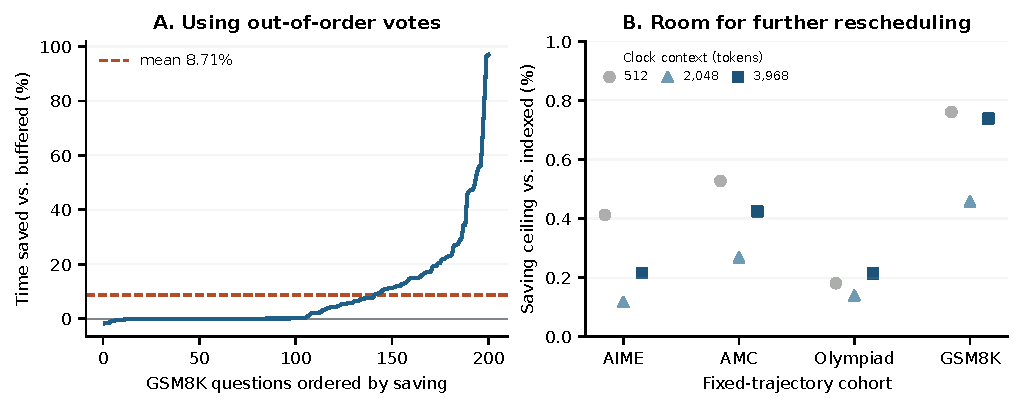
\includegraphics[width=.96\textwidth]{evidence.pdf}
\caption{Two comparisons under fixed service clocks. Left, per-question change in modeled time from using all indexed votes for admission instead of only the contiguous prefix, at the 3,968-token clock. The dashed line is the question mean. Right, the ceiling on mean time savings of any legal scheduler over indexed greedy in each cohort, computed separately with each A800 width-price curve. The two vertical axes have different references and scales.}\label{fig:evidence}
\end{figure*}
Figure~\ref{fig:evidence} shows the heterogeneity in the admission comparison. The typical question changed little, while a subset benefited enough to lift the mean. Across all four cohorts every fixed clock left less than one percent average headroom after indexed admission.

\subsection{Controlled measurements in a decoding engine}
On the 24 OlympiadBench questions we paired the indexed and buffered policies on an A800 by holding the per-path generation lengths and released votes fixed. Each policy issued real vLLM requests and returned on certification or quota exhaustion. We separately sampled natural answers with matched path seeds. In the fixed-work runs the two policies performed every reservation, launch, completion and cancellation at the same engine step on all 24 pairs. Each generated 1,114,134 tokens in total. Their average wall times differed by 0.14\% despite identical dispatches. The natural comparison gave 0.12\% savings (95\% question interval $-0.06$ to 0.32\%). Each condition was timed once per question, so this analysis cannot isolate cross-session timing variance. On fixed votes nine decisions were certified at or before fourteen launches. All 24 capped answers agreed with the full sixteen-vote output, twelve of them by joint abstention. Eleven answers matched the integer gold value.

\paragraph{Do the replay results transfer to new device panels?}
We independently generated sixteen GSM8K panels with Qwen2.5-1.5B-Instruct in BF16 on the A800, selecting questions by hash before generation. Matching the exact question texts to the rollout publisher's benchmark file showed that two pilot questions also appeared among the 200 archived panels (\texttt{gsm8k\_497} and \texttt{gsm8k\_695}). All sixteen sets of device trajectories were freshly generated. We obtained a sixteen-path reference per question, a pair of runs with the reference lengths and votes fixed, and a pair with natural sampling and matched per-path seeds. We counterbalanced the condition order. All arms used temperature 0.7, top-$p$ 0.95 and a 384-token cap. We used a balanced final boxed integer as the vote and treated invalid or truncated generations as abstentions. Each timed panel starts after a separate warmup and ends after cancellation and device synchronization. The primary measure was the question-mean fixed-work wall-time saving. We required a point estimate of at least 2\%, a positive lower limit in 20,000 paired question bootstrap draws, and at least one different dispatch.

\begin{table}[tb]\centering
\caption{Paired A800 measurements on 16 GSM8K questions. Changed counts questions with any difference in indexed launch steps. Correct gives the number of correct final outputs per arm. Intervals resample questions from one device session.}\label{tab:a800pilot}
\small\setlength{\tabcolsep}{3pt}
\begin{tabular}{lrrrc}\toprule
Generation & Changed & Saved (\%) & 95\% interval & Correct\\\midrule
Fixed & 4 & 0.55 & [$-0.03$, 1.29] & 10/16\\
Natural & 5 & 0.48 & [$-0.04$, 1.30] & 9/16\\\bottomrule
\end{tabular}
\end{table}
The fixed-work pilot missed the prespecified practical threshold (Table~\ref{tab:a800pilot}). In that condition the indexed engine took fewer steps on three questions and tied on thirteen. Its 15,560 total steps generated 55,429 tokens, compared with 15,670 steps and 55,490 tokens under buffered admission. Under natural sampling both policies returned the same answers on every question, while the indexed policy emitted 176 more tokens overall. Including the separate reference, all eighty recordings used 289,877 generated tokens.

After the pilot, we ran the 3,968-token replay clock on those same sixteen fixed panels. It predicted a 0.60\% question-mean saving and correctly identified the four dispatch differences and twelve unchanged schedules. The archive-derived 8.71\% estimate had come from a different model and generation protocol. The matched-panel comparison shows that a change in the trajectory population can reduce the opportunities for earlier launches. One pilot with one timed pair per question leaves the session-to-session variance unmeasured.

\subsection{Does a longer output limit increase the value of indexed admission?}\label{sec:cap}
An output limit can affect two parts of a voting schedule. Truncating a long path frees its slot sooner. Discarding the unfinished answer changes the votes available to admit later requests. To separate these effects, we intervened on the 200 archived GSM8K panels after the initial analysis. The original generation limit was 31,744 tokens. Among 3,200 paths, 550 from 172 questions exceeded 384 tokens, while 146 from 87 questions reached at least 1,024. Clipping their work to 384 while keeping their original votes reduced the mean indexed-over-buffered saving from 8.71\% to 2.62\% at the 3,968-token clock. Keeping the work and replacing only the affected votes by abstentions gave 9.64\%. Applying both changes gave 2.81\%. Thus clipping the long paths accounted for most of the reduction in this archive. The separate interventions use counterfactual terminal votes to isolate each change.

We next compared limits of 384 and 1,024 with the integer parser used on the device. On the same 200 archived questions the modeled mean saving rose from 2.84\% to 7.41\%, a difference of 4.57 percentage points. With the archive parser, the corresponding means were 2.81\% and 7.62\%. We fixed the protocol for a directional test on the A800. We excluded all 200 archived questions and all 16 pilot questions, then selected 32 by a frozen text hash among the 1,105 remaining GSM8K questions. The protocol specifies sixteen reference generations per question, capped at 1,024 tokens, from Qwen2.5-1.5B-Instruct. The short reference truncates these same paths at 384. A path reaching the applicable cap abstained.

At each cap the two gates run with the same fixed path lengths and votes. Four condition orders balance the timed comparisons across questions. For question \(q\) and cap \(c\), let \(s_{q,c}=1-T_{\mathrm{indexed},q,c}/T_{\mathrm{buffered},q,c}\), where \(T\) measures synchronized wall time. Our primary outcome was the question mean of \(s_{q,1024}-s_{q,384}\). The frozen analysis uses a two-sided 95\% bootstrap interval with 20,000 draws of 32 paired questions. The separate practical criterion at 1,024 tokens required at least 2\% saving against buffered admission at that cap, a positive lower confidence limit and at least one changed dispatch.

The short-cap saving was 0.86\% (95\% interval $-0.33$ to 2.23\%) and the long-cap saving was 1.30\% (0.33 to 2.39\%). Their paired difference was $+0.44$ percentage points (95\% interval $-0.79$ to $+1.84$). The trial leaves the directional hypothesis unresolved. The long condition had a positive lower endpoint but fell short of the prespecified 2\% useful saving. Figure~\ref{fig:cap} retains all question-level slowdowns and savings.

Only 35 of the 512 newly sampled paths reached 384 tokens, and two reached 1,024. On 20 of 32 questions the two limits gave identical fixed work and votes. Dispatch changed between gates on five questions at the short cap and seven at the long cap. The indexed gate needed fewer engine steps on three questions at each cap. Replaying the measured paths classified all 64 question--cap dispatch comparisons correctly. Its estimated change in saving was $-0.32$ percentage points, opposite in sign to the wall-time point estimate. Thus correct predictions about which questions take different scheduling actions can coexist with uncertainty about the wall-time difference. The single device session does not separate session variation from a persistent timing effect. Appendix~\ref{app:cap} reports the absolute costs at both output limits.


\paragraph{A prediction before device validation.}
On Qwen2.5-1.5B-Instruct, a separate A800 calibration gave step costs of $4.711,4.611,4.810$ ms at widths one through three. When all requests of prescribed lengths $(256,128,128)$ must finish, immediate launch costs $128(c_3+c_1)$ in the model. Deferring the third request until the second finishes costs $256c_2$. We sealed a predicted saving of 3.13\% before starting a fresh engine process. Twelve paired measurements gave a median whole-panel saving of 2.46\% (within-session interval 2.38--2.61\%). For two equal lengths $(128,128)$, serial execution took 102.63\% longer than parallel execution against a prediction of 104.30\% longer. Both contrasts met the prespecified two-percentage-point tolerance. On the first three paths of 200 archived questions, staging won on 66. Choosing the faster action with knowledge of all lengths saved just 0.364\% on average under this clock. Appendix~\ref{app:transfer} gives individual blocks and timing boundaries.

\section{Related work}
Self-consistency aggregates multiple model-generated reasoning paths \citep{wang2023sc}. Recoverable-winner tests characterize which final outcomes are compatible with the votes observed so far, including tie-aware certificates \citep{recover}. We use the conservative strict-margin test and ask how many irrevocable launches are admissible \emph{before} the next certificate arrives. Fixed-width microbatches already enforce an overrun bound of their width minus one when they check at each barrier. In a retrospective AIME replay under unit prices, indexed admission saved 47.38\% against a width-two barrier that satisfies the same budget. The rolling buffered gate already saved 40.45\% against that barrier. Both gates in our main comparison refill asynchronous slots and check all completions for stopping, isolating the information used to admit later requests.

Classical curtailed sampling also ends a sampling plan when remaining observations cannot change its decision \citep{curtail}. Delayed-response sequential tests account for recruited participants whose outcomes have yet to arrive \citep{Hampson_2012}. Parallel ranking and selection can pre-index samples and present their values in index order to a screening procedure \citep{Ni_2017}. Competitive Boolean function evaluation asks which tests to perform and compares their cost with a certificate on a realized input \citep{cicalese}. Sequential batch testing accounts for batch setup costs and statistical failure models \citep{Segev_2022,yang2024testing}. Our work fixes the launch order and measures time while concurrency changes the rate of every active query. It combines certificate requirements with unavoidable service to earlier indices.

Async test-time scaling already uses freed slots, calibration and intermediate feedback \citep{duchess,atts,mars}. SPEX uses a hardware roofline to allot speculative reasoning branches and exploits reward signals to choose expansions \citep{zhong2026spex}. SpecScale delays verification to form larger batches \citep{jeong2026specscale}. Delayed replication studies when to fork redundant servers given service-time distributions \citep{badita2020stragglers}. These contributions establish practical reasons to control concurrency. Our comparison fixes each branch's work and vote and imposes an instance-wise limit relative to its realized serial prefix. It identifies how much a timing intervention can recover after retaining all completed votes for admission.

Profile scheduling treats processor availability as input \citep{dolev1985profile,liu1997variable,liu1995det}. Our profile is the number of busy slots under a policy. Predictability under shorter job requirements \citep{cucu2010} and alternative enabling sets in AND/OR precedence models \citep{moehring2004} have classical antecedents. On fixed labels a logical predicate can encode which completions permit another start. A single fixed predecessor set on the original jobs can fail even at the same time with two idle slots (Appendix~\ref{app:precedence}). Rearrangement and majorization are established tools \citep{chang1993rearrangement}. Here time compression and the shrinking width allowed by returned votes give a comparison with the rearranged busy widths of every admissible policy.

The subset-capacity inequalities in Theorem~\ref{th:floor} have a classical discrete counterpart. In a zero-one service matrix, a row with sum \(k\) can contribute at most \(\min(k,m)\) units to any \(m\) columns. Summing these capacities gives the necessity direction of the row-sum and column-sum majorization theorem of \citet[Thm.~2.1]{ryser1957}. Here each interval has a duration and a width-dependent price. The contribution of \eqref{eq:work} is to derive the column demands from the vote sets sufficient to end computation and the service owed to earlier requests that cannot be paused. General polytope scheduling also integrates feasible service rates over time \citep{jaeger2025}. Its weighted job-completion objective and selectable rate allocation differ from the time to obtain a vote certificate under equal rates for the active jobs.

\section{Scope and conclusions}
Some evaluations require every sample. The Language Model Evaluation Harness can log all 64 responses in its GSM8K self-consistency task \citep{eleuther2024gsm64}. A scheduler serving that interface must return all requested samples. The same occupancy comparison applies when all paths must finish in fixed launch order (Appendix~\ref{app:major}). In early-stopped physical evaluations, \citet[App.~H.4]{recover} charge each request already issued at a microbatch boundary. At batch width $m$ that policy can spend up to $m-1$ calls beyond the serial stopping point.

The operator chooses which guarantee to offer. Existing frameworks implement absolute call limits \citep{pydanticlimit,langchainlimit}, while the prevalence of a per-question serial-relative allowance remains unmeasured. In a retrospective comparison on 200 archived GSM8K questions, eager refill subject only to $Q=14$ actually exceeded $K+1$ on 93 questions. Enforcing $B=1$ saved 0.985 starts per question and increased modeled time by 20.76\% on average. On the 32 device-generated path sets at the 384 and 1,024 limits, the same replay saved 1.47 and 1.53 starts per question at mean time costs of 0.42\% and 0.16\%, respectively. A service that primarily values average resource use or cancellation counts has a different admissible class.

The occupancy argument also applies to ordered candidates that return a terminal pass or fail, when the service seeks $r$ passes and promises zero excess starts relative to serial verification (Appendix~\ref{app:rpass}). The bounds assume common progress across active paths. Long prefill, imbalanced KV caches or interference from another tenant can violate that assumption. Evaluating a shared service requires matched arrival streams, queueing measurements and costs associated with continuing or aborting work.

At zero extra starts, fixing the slot count and width prices gives an exact worst-case ratio across all panel sizes, quotas, works and votes. It remains an upper bound for any fixed size and quota. With one extra start the attainable saving depends on the votes and work. On the panels studied here, the work forced by each certificate left little room for timing changes. On archived GSM8K trajectories most of the gain over prefix-only admission came from counting out-of-order votes. Knowing their exact positions contributed a much smaller gain.

\FloatBarrier
\section*{Impact Statement}
Budget guarantees can help operators bound speculative model calls. Waiting may increase user latency or alter the work spent on other requests. Changes to answer quality, tenant fairness and actual fees depend on deployment and on the generation and cancellation interfaces.
\section*{AI Disclosure Statement}
OpenAI Codex helped formulate the problem and derive the proofs, wrote the main simulator and engine driver, ran the experiments, analyzed the data and prepared the initial manuscript. Separate verification programs enumerated small panels and reconstructed the timing comparisons from archived engine events. The literature audit records the editions, theorems and pages inspected and the limits of the search. The supporting material includes proofs, code and input fingerprints.
\bibliographystyle{icml2027}
\bibliography{refs}
\clearpage\appendix\onecolumn
\section{Zero excess starts fix the total amount of executed work}\label{app:zero}
At a strict return let \(S\) contain the \(s\) completed votes, with winner \(a\). At the last dispatch the observed votes \(S_0\) formed a subset of \(S\). We construct an input compatible with \(S_0\) on which the serial run locks by index \(s\). Keep the observed votes of \(S_0\) in positions \(1,\ldots,s\), assign every other position of that prefix to \(a\), and honor all other known votes beyond \(s\). The resulting prefix's multiset can be formed from \(S\) by retaining the specified observations and replacing the remaining votes by \(a\). This cannot reduce \(a\)'s lead. The prefix therefore certifies \(a\) strictly. With \(B=0\), \(J\le s\) at the last dispatch. Since every completion has launched, \(s=J\). On the realized input, these \(J\) finished paths form a serial prefix. Its certificate implies \(K\le J\), and the allowance imposes \(J\le K\). If the service instead exhausts its quota without a strict certificate, a smaller locking prefix would also lock the full quota prefix, so \(K\ge Q\). These cases prove invariance of \(\sum_{i=1}^{\min(K,Q)}w_i\) under all compliant schedules, including when paths have schedule-dependent completion times through their common service clock.

\section{Occupancy majorization for an arbitrary slot count}\label{app:major}
At a reachable zero-overrun history let \(h(S)=|S|+m(S)\) where \(m(S)\) counts the fewest further completions that can produce a strict lock or exhaust the full \(N\)-vote panel. The absolute quota separately limits further work to \(Q-|S|\) completions. Filling \(m\) further outcomes with the current leader gives such a decision, so retaining observed indices in the first \(h\) positions and assigning its other positions to the leader constructs a compatible \(K\le h\). Thus \(M\le h\). On a zero-allowance history, all previously admitted indices are at most \(M\), by the monotonicity of \(M\). Conversely a compatible serial locking prefix of length \(M<N\) contains all observations and must include at least \(m\) additional positions. If \(M=N\), exhaustion gives the same inequality. Hence \(M=h\). The width permitted just after replenishment is \(\min(P,m(S),Q-|S|)\), a nonincreasing function of newly observed information since each vote decreases the remaining count by one and changes the margin by at most one.

In particular, $m=\min\{R,\max(0,\lfloor(R-g)/2\rfloor+1)\}$, where $R=N-|S|$ and $g=\gap(S)$. This includes the terminal boundary. The absolute quota and slot cap apply separately.

Fix votes and let $w'_i\le w_i$ for every job. Greedy on $w'$ starts and finishes each job no later in virtual time than any admissible comparator on $w$. Induct on the comparator's launches. Its previously completed paths started no later on the shortened greedy execution and needed weakly less work. Thus at the comparator's next launch the shortened greedy run includes all the observations used for admission, so it has already filled to at least the same cumulative frontier. If shortened greedy already terminated, the common prefix result shows that it already finished the same jobs. In particular, greedy on $w'$ includes all completions of greedy on $w$ at the same virtual time. The nonincreasing active-width cap derived above yields $h_{G,w'}(t)\le h_{G,w}(t)$, with both profiles set to zero after their respective decisions.

For a schedule $A$ of finite duration $D$, let $E$ be any union of intervals and fix $0<\epsilon<1$. Reparameterize its timeline by the strictly increasing map
\[
 \phi_\epsilon(t)=\int_0^t (\mathbf{1}_E(u)+\epsilon\mathbf{1}_{E^c}(u))\,du .
\]
Transform every start $s_i$ and finish $e_i$ and set $w'_i=\phi_\epsilon(e_i)-\phi_\epsilon(s_i)>0$ for its completed paths. Keep the work of unlaunched paths unchanged. Running the same jobs between transformed endpoints with unit virtual rate realizes that shorter input. All event orders, simultaneous returns, slot counts and vote histories at dispatches are preserved. Write $D_\epsilon=\phi_\epsilon(D)$. On this input greedy completes by $D_\epsilon$ and executes the same total work as the transformed schedule. Therefore
\[
 \int_E h_A+\epsilon\int_{[0,D]\setminus E}h_A
 =\sum_{i\le J}w'_i=\int_0^{D_\epsilon}h_{G,w'}(u)\,du
 \le \int_0^{D_\epsilon}h_{G,w}(u)\,du .
\]
The last profile is bounded by $P$ and independent of $\epsilon$. Letting $\epsilon$ decrease to zero proves \eqref{eq:major}, without introducing zero-work jobs. For $E=\{h_A>j\}$ subtract $j|E|$ from both sides and upper-bound the right side by $\int (h_{G,w}-j)_+$. Thus greedy maximizes this integral for every threshold. Put $\theta_j=2c_j-c_{j-1}-c_{j+1}$. The discrete identity $c_k=c_1k-\sum_{j=1}^{P-1}\theta_j(k-j)_+$, equal total work, and $\theta_j\ge0$ give $T_G\le T_A$.

For an ordered panel that must complete all $N$ paths, the same comparison follows with cumulative frontier $\min(N,|S|+P)$ and greedy width $\min(P,N-|S|)$. These two quantities are respectively nondecreasing and nonincreasing as completions arrive, and every scheduling policy executes exactly the same work. The shortened-input comparison and time compression therefore give \eqref{eq:major} and optimality under concave prices for this fixed-panel objective.

If $\theta_j<0$ for any $j<P$, take any even $N\ge\max(2j,P)$, all votes equal and quota $Q=j+1$. No set of $j$ votes certifies, allowing all $Q$ launches at the outset. Give the first $j-1$ jobs work two and the following two work one. Greedy takes $c_{j+1}+c_{j-1}$. A policy starting $j$ jobs and replenishing at the short job's finish takes $2c_j$. At $j=1$, $c_0=0$ accounts for the already completed greedy run. This establishes necessity. As a finite independent check, a dynamic program maximizing each threshold over every integer-time launch choice verified all 4,488 comparisons in 1,416 configurations at four through eight slots, representing 1,651,840 complete histories.

\subsection{Sharp price ratios for nonconcave clocks}\label{app:sharp}
Let $\gamma=\max_{1\le k\le P}\widehat c_k/c_k$. The upper bound in the main text holds on every panel, and when $\gamma=1$ it is exact. For $\gamma>1$, a maximizing $j$ lies strictly between two contact widths $0\le a<j<b\le P$ of the piecewise-linear concave majorant. The value $\widehat c_j$ is the height of their chord. Write $S=\mathrm{lcm}(b-a,j-a)$ and $L=S/(j-a)$. Choose a multiple $d$ of $P$ with $d>S+a+P$. Use $N=2(d+b-1)$ and $Q=d+a+S$. The first $d$ paths have work $\epsilon>0$ and vote A. The next $a$ have work $L$, the following $S$ have work one, and these $a+S$ paths all vote B. All remaining votes can be chosen arbitrarily.

Both schedules execute the first $d$ paths in full batches of $P$. After $s\le d-P$ prefix completions the admissible in-flight allowance before quota and slot caps is $d+b-s$, at least $P$. After all $d$ prefix votes arrive it is exactly $b$. Each suffix completion reduces the number of unresolved votes and the A lead by one. The inequality on $d$ keeps A ahead, so the vote constraint continues to allow $b$ in-flight requests throughout the suffix. Neither policy can certify early, and they finish all $Q$ paths. Greedy first starts all $a$ long jobs and fills the other $b-a$ slots with short jobs for $S/(b-a)$ virtual steps. It then runs only the long jobs until $L$. For $a=0$ the second segment costs zero because greedy is already done. Its suffix cost is
\[
 \frac{S}{b-a}c_b+\left(L-\frac{S}{b-a}\right)c_a
 = L\left(\frac{j-a}{b-a}c_b+\frac{b-j}{b-a}c_a\right)=L\widehat c_j .
\]
The comparator starts the long jobs and keeps only $j-a$ short jobs in flight until $L$, at cost $Lc_j$. The integrality of both short-job batch counts follows from the choice of $S$. The common prefix cost is $(d/P)c_P\epsilon$. Letting $\epsilon$ decrease to zero yields a greedy-to-comparator ratio approaching $\widehat c_j/c_j=\gamma$. Since $T_{\rm opt}\le T_A$, this establishes the matching lower bound on the supremum. The construction was also replayed with the indexed gate for all 210 triples $a<j<b$ at slot counts two through eight.

To see why repricing fixes the execution, set $N=8$, $Q=4$, $P=3$, $B=0$, with unit work on the first four paths and prices $(10,11,13)$. Four starts are safe even before any votes return. Run the first two together. Run the next two together if the first pair finishes in less than $11.25$ wall-time units, and serially otherwise. At the original prices the schedule costs $22$. Repricing that virtual trajectory under the concave majorant $(10,11.5,13)$ gives $23$. Executing the same wall-time rule anew at those prices instead gives $11.5+20=31.5$. The proof uses the repriced trajectory.

\section{Enumerating the certificate-work relaxation}
Use one bit per path among the first \(Q\). A terminal mask must be a strict certificate or the full exhausted quota. For any completed \(j\), discard a mask lacking an \(i<j\) with \(w_i\le w_j\). Also test the largest completed index \(j\): even if every other vote in the mask had already arrived, \eqref{eq:f} must have permitted the launch through \(j\). These necessary tests leave a superset of attainable masks. Compute the vector of lower bounds in \eqref{eq:lp} for each retained mask. Componentwise larger requirement vectors can be dropped when minimizing across masks.

The resulting LP has only \(P\) occupancy variables. Combine the \(m=1\) row with the virtual time requirement and use the total-work constraint for \(m=P\). Write the resulting requirement vector as \(b\). Its dual is
\[
 \max_{y\ge0} b^\top y
 \quad\text{subject to}\quad
 \sum_{m=1}^P\min(k,m)y_m\le c_k\quad(k=1,\dots,P).
\]
We enumerate its vertices with exact rational arithmetic, then choose the smallest optimum across the masks. Its cost grows exponentially with the absolute quota through the number of candidate terminal sets. The certificate calculation can run offline on traces and leaves the online index scan unchanged.

\paragraph{An independent check with continuous launch delays.}
For integer work there exists an optimal schedule which starts only at integer virtual times. To see this, fix the order of the starts and completions through termination, including inequalities that keep unfinished requests' natural end after the deciding event. Write \(s_i\) for job \(i\)'s start. Its natural completion is \(s_i+w_i\). All imposed event orders give difference inequalities with integer offsets between start variables. Remove zero-width idle periods and set \(s_1=0\). For a schedule no slower than \(G\), all starts can be bounded by \(\lceil T_G/\min_k c_k\rceil\). Inside this order region the objective sums linear differences between the event times at each width. The closure is a bounded difference-constraint polyhedron, whose vertices have integral coordinates: tight equalities determine the start variables by integer differences along an anchored forest. A linear objective attains its minimum at one of the vertices. When a vertex merges events, process simultaneous completions before launches. The observations contain all those required for the original dispatches. If a decision now occurs earlier, remove subsequent dispatches. This operation preserves feasibility and does not increase elapsed time. There are only finitely many event orders. This proves existence on the integer grid even when the original competitor may use a continuous timer.

We enumerated safe schedules by dynamic programming with independently enumerated unseen votes. Across 11,776 configurations with three or four paths, two or three slots, integer work in \(\{1,2\}\), multiple budget settings, and increasing, flat or nonmonotone width costs, all work bounds held. The lower bound matched the exact optimum in 9,390 configurations and improved on the virtual-time-only floor in 6,537. Waiting could beat greedy in 3,112. A second oracle admitting starts on a half-unit grid gave the same optima. A distinct test of the zero-allowance theorem included 17,640 panel settings and 70,560 affine-price comparisons. These checks serve as implementation audits in addition to the proofs.

\section{What can a timer guarantee?}\label{app:timer}
At a completion event, some combination of the active votes may be sufficient to decide. Waiting for the next completion protects those requests from additional interference. It can also delay a short decisive vote until a slow request returns. Take sixteen A votes with four slots, \(Q=14,B=1\), and works \((L,2,1,1,\ldots,1)\). By virtual time 3, eight A votes have returned and path 1 still runs. Path 10 may safely start. Greedy obtains the ninth vote and decides at time 4. A policy that postpones this last start until the next completion decides at \(L\). The ratio grows without bound.

\begin{theorem}[Bounded waiting]\label{th:wait}
If a safe policy \(D\) fills to the indexed frontier except during a finite union of withholding intervals of realized total virtual duration \(H\), and refills at their right endpoints, then \(V_G\le V_D\le V_G+H\). The upper bound is sharp with \(N=16,P=4,Q=14,B=1\).
\end{theorem}
\begin{proof}
Let \(I\) be the union of the withholding intervals and set \(C(t)=t-|I\cap[0,t]|\) on \(0\le t\le V_D\). If \(C(V_D)=V_D-H\le V_G\), then \(V_D\le V_G+H\) directly. To cover the remaining case, for any \(0\le u<C(V_D)\) define \(\phi(u)=\sup\{t\le V_D:C(t)\le u\}\). At a collapsed interval this chooses its right endpoint, when \(D\) refills if still running. We have \(u\le\phi(u)\le u+H\) and \(\phi(v)-\phi(u)\ge v-u\) for \(u\le v\). By induction, each launch made by \(G\) by \(u\) has occurred under \(D\) by \(\phi(u)\), unless \(D\) has returned. Indeed, previously launched paths that finished under \(G\) have received enough virtual time to finish under \(D\). Their votes allow the same cumulative launch count, and at \(\phi(u)\) policy \(D\) fills to its frontier. When \(V_G<C(V_D)\), take \(u=V_G\). Those observations give a lock or quota exhaustion, so \(V_D\le\phi(V_G)\le V_G+H\). The lower bound follows from virtual launch dominance up to return. In the preceding example a single wait for \(H<L-4\) delays the decision from 4 to \(4+H\).
\end{proof}
This bound limits extra virtual time. A change in active width also changes its wall-clock price. Appendix~\ref{app:clock} gives a physical upper bound in terms of \(H\) and the measured variation of adjacent prices.

\section{Interpreting a cap on waiting in wall time}\label{app:clock}
Let \(c_{\max}=\max_k c_k\), and let \(L_+=\max(0,\max_{k<P}(c_{k+1}-c_k))\) and \(L_-=\max(0,\max_{k<P}(c_k-c_{k+1}))\). For \(P=1\) set both variation terms to zero. Suppose the nonterminal schedule always keeps a path active. If \(J\) and \(C\) paths have launched and completed in greedy by its decision, then a scheduler that withholds legal starts for a union of virtual intervals of total duration \(H\) satisfies
\[
          T_D-T_G \le H\big(c_{\max}+ C L_+ + J L_-\big).
\]
The resulting wall bound permits either ordering of \(T_D\) and \(T_G\). Theorem~\ref{th:wait} follows on each realized sequence of adaptive postponements or private random draws.

Write \(J_A(t)\) and \(C_A(t)\) for launches and completions by virtual time \(t\), taking zero at negative times. On \(0\le t<V_G\), virtual-time dominance bounds the two counts for \(D\) above by those for \(G\). The compressed-clock proof also bounds them below by the corresponding counts for \(G\) at \(t-H\). Integrating the launch deficit therefore costs at most \(JH\): each launch contributes for at most \(H\) time units. The completion deficit similarly integrates to at most \(CH\). At each time occupancy is launched count minus completed count, so excess width under \(D\) is no larger than the completion deficit and its shortfall is no larger than the launch deficit. Bounding the resulting price changes by \(L_+\) and \(L_-\) gives at most \(H(CL_++JL_-)\) extra elapsed time up to \(V_G\). The remaining virtual tail has length at most \(H\) and price at most \(c_{\max}\). An independent small-panel check evaluated the virtual bound on 24,768 allowed schedules or schedule comparisons and attained its upper limit on 3,096.

\section{Clock envelopes at positive allowance}\label{app:box}
The certificate bound $L(c)$ is an infimum of linear functions of the price vector $c$ over a common set of occupancy vectors, so it is concave. For a question with several panels, sum these bounds and the corresponding greedy times to obtain a concave lower bound $L_q(c)$ and a positive linear denominator $G_q(c)$. For $c$ in a box, write $c=\sum_v\lambda_v v$ using its corners. The ratio $L_q(c)/G_q(c)$ is bounded below by a weighted average of $L_q(v)/G_q(v)$, with weights proportional to $\lambda_vG_q(v)$. Taking each question's worst corner and then averaging gives an upper bound on the question-mean saving for every shared fixed clock in the box. Four widths require sixteen corners. If the within-question prices vary while remaining inside the box, charge the certificate bound at the componentwise minima and greedy at the maxima. The calibration measures eight block averages at each width in one session. The resulting envelope is a conditional sensitivity calculation.

\section{Admission with partially indexed votes}\label{app:bag}
For a prospective launch $j$, the serial-relative promise rules out a decisive prefix before $j-B$. Test $t=\max(0,j-B-1)$ because a strict lock remains a lock after later votes arrive. At this prefix maximize the possible lead among all vote assignments consistent with the information exposed to the gate. The indexed rule fixes all observed indices in the prefix, and fills each missing position with a vote for their current leader. The unordered gate knows the mask of completed positions and the multiset of all returned votes but forgets their pairing. Enumerate which sub-multiset of returns could occupy the completed positions in the prefix, then fill the missing positions to maximize the lead. The prefix-plus-multiset gate further fixes the initial contiguous returned votes in their observed positions before performing this enumeration. A launch is safe if this maximum is at most $N-t$. Physical slots and the absolute quota apply to all three rules. The comparison concerns assignments compatible with a single snapshot. A gate that retains its earlier observations could infer additional associations. The fully indexed decision can maintain the cumulative tally through $t=\max(0,J-B)$ together with the number of completed positions in that prefix. Only the last $B$ launched positions can lie beyond $t$, so their individual returns suffice in addition to label totals and the engine's active-request ledger. When $J$ grows by one, at most one such record enters the cumulative tally. It uses the same fixed trajectories and terminal rule as the index-aware policy.

\section{Inputs, statistics and sources of variation}\label{app:data}
The AIME, AMC and GSM8K traces came from the public \href{https://huggingface.co/datasets/reasoning-cues/rollouts-qwen4b/tree/b8c33b85a1a6cdfb23b06a5f9d696f52950780e4}{Reasoning Cues Qwen3-4B-Base archive} at revision \texttt{b8c33b85}. For AIME the fixed within-question shuffle produced two disjoint sixteen-path panels per question. The AMC analysis used the second of two distinct draws for each question. For GSM8K the parser removed whitespace from the last balanced boxed answer and recorded missing or truncated answers as abstentions. Shard names matching the first-draw unsteered pattern were sorted by the SHA-256 digest of a fixed namespace followed by the published path. The parser, eight selected shard object IDs and protocol were frozen before fetching their contents. All 3,200 selected trajectories belonged to complete panels. No extra model calls were used to forecast future votes in this evaluation.

For each of the 200 GSM8K questions, the paired saving was one minus the indexed-to-comparator time ratio for the admission comparisons. For each interval we sampled 200 questions with replacement and took the 2.5\% and 97.5\% quantiles of the resulting question means. The prespecified comparisons used 10,000 resamples with seed 19431. The two retrospective comparisons against the unordered and prefix-plus-multiset gates used 20,000 resamples with seed 651. These intervals treat questions as exchangeable, conditional on the selected shards and generation seeds. Published trajectory text and indices do not supply a complete execution environment for reconstructing the original sampler. Generated work includes partial canceled paths. A path count, a generated-token count, an invoice and an entire question's response time are distinct resources.

All eight selected shards had positive mean indexed-versus-buffered savings. Leaving out each shard in turn gave a question-mean saving ranging from 8.15\% to 9.23\% at 3,968 tokens.

\begin{table}[htbp]\centering
\caption{GSM8K sensitivity to a fixed width clock, in question-mean percent time saved. References are the buffered gate in the first row and indexed greedy in the remaining rows.}\label{tab:sens}
\begin{tabular}{lrrr}\toprule
Policy & 512 & 2,048 & 3,968\\\midrule
Indexed versus buffered & 8.934 & 8.880 & 8.709\\
Repeated conditional wait & $-76.040$ & $-75.005$ & $-73.244$\\
First conditional wait, eight-step cap & $-0.307$ & $-0.302$ & $-0.300$\\
First eligible wait, eight-step cap & $-0.229$ & $-0.225$ & $-0.224$\\
Hindsight best single wait & 0.103 & 0.100 & 0.115\\\bottomrule
\end{tabular}
\end{table}

The best-single-wait enumeration includes every eligible event on greedy's path because no prior launch differs before a first deviation. This enumeration excludes schedules which intentionally postpone more than once or which choose arbitrary continuous delays. Its optimum is directly realizable with future information, whereas the certificate-work relaxation bounds a larger action class without requiring its optimizer to correspond to a real schedule.

\section{Paired output-limit experiment on the A800}\label{app:cap}
The 32 eligible question hashes and the order of the four runs per question were fixed before the first model output. We used a separate seed namespace for this study and took every path from the same 1,024-token reference per question. The two policies returned identical answers within each cap. Across caps, the answer changed on two questions. Each question contributed one timed pair at each cap within a single device session. At 384 tokens 15 questions saved wall time and 17 took longer. At 1,024 tokens 22 saved time and 10 took longer. The paired estimates in the main text average individual question ratios. The summed costs below also include work already performed by paths canceled at return.

\begin{table}[htbp]\centering
\caption{Absolute cost of running each fixed-work policy on all 32 questions. Correct and certified count question-level decisions. Request starts and generated tokens include canceled requests. References for the paired savings are the buffered row at the same cap.}\label{tab:abscap}
\small\begin{tabular}{rlrrrrrr}\toprule
Cap & Gate & Wall time (s) & Steps & Generated tokens & Starts & Correct & Certified\\\midrule
384 & Indexed & 153.33 & 26,895 & 95,159 & 384 & 26 & 26\\
384 & Buffered & 154.77 & 27,159 & 95,303 & 384 & 26 & 26\\
1,024 & Indexed & 158.22 & 27,578 & 96,855 & 380 & 27 & 27\\
1,024 & Buffered & 161.02 & 27,834 & 96,611 & 380 & 27 & 27\\\bottomrule
\end{tabular}\end{table}
Both gates took longer in absolute time at the larger output limit. A change in relative saving compares indexed with buffered at each cap and allows their absolute times to increase. Including the 32 full references, the 160 timed panels generated 515,582 tokens in 835.24 seconds of synchronized panel time. The full 16-vote plurality answered 27 of the 32 questions correctly under each cap.

\begin{figure}[htbp]\centering
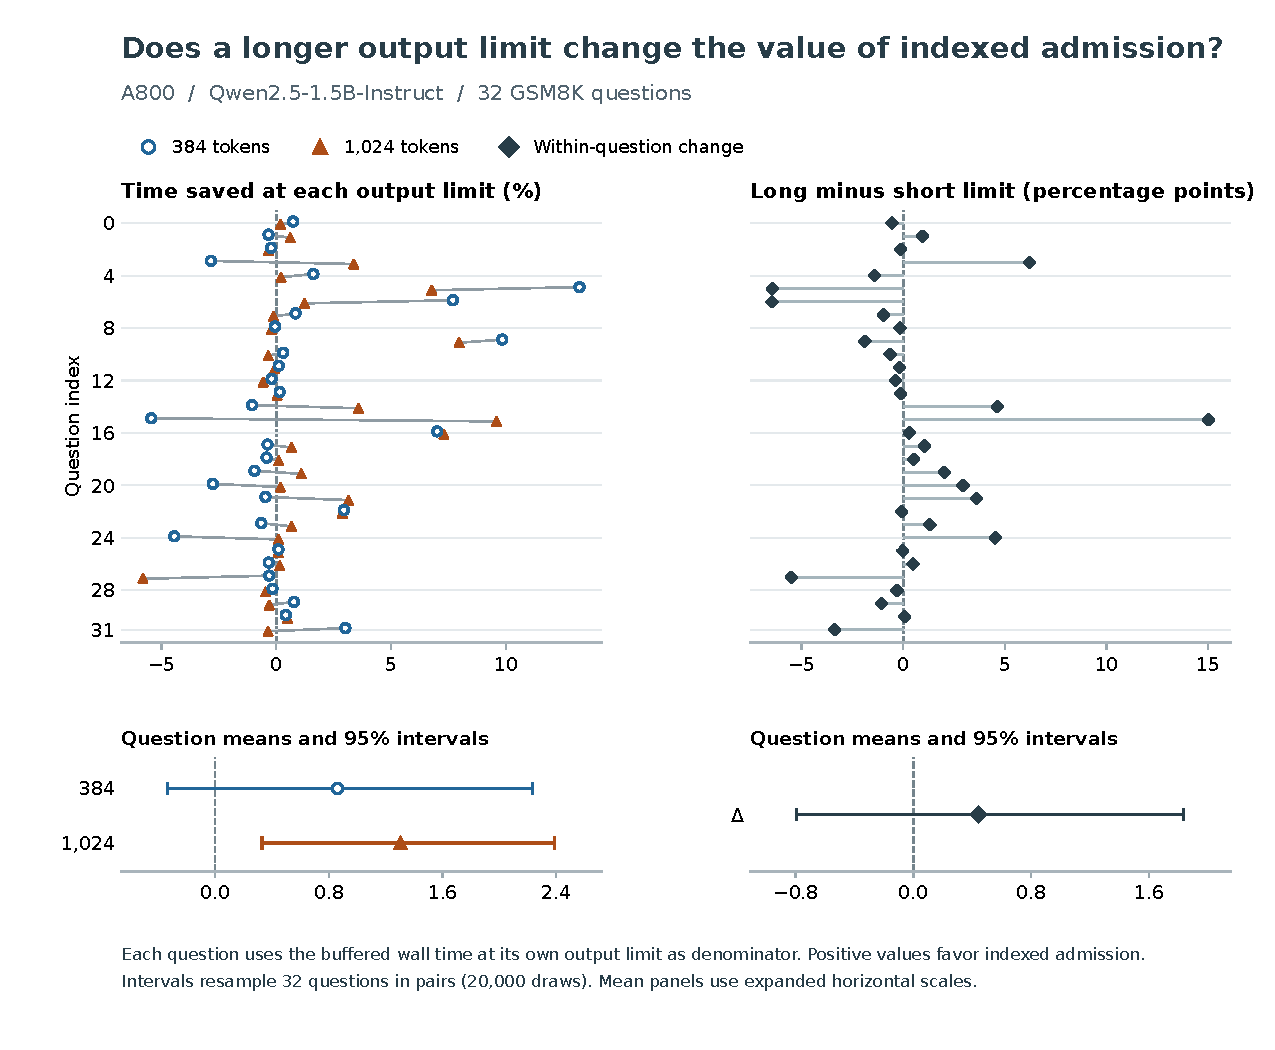
\includegraphics[width=.97\textwidth]{cap-comparison.pdf}
\caption{Per-question savings in synchronized A800 wall time. Each observation compares the indexed and buffered gates under one output limit. The right-hand contrast subtracts the short-cap saving from the long-cap saving on that question. The lower panels show question means and paired 95\% bootstrap intervals on expanded axes.}\label{fig:cap}
\end{figure}
\section{Two comparisons with classical scheduling}\label{app:precedence}
First consider a fixed prerequisite set on the original jobs. A job becomes eligible once every job in its prerequisite set has finished. Set $(N,P,Q,B)=(9,5,9,0)$. Start job 1 at time zero with work 10. Give jobs 2 through 5 works $(4,3,2,1)$ and votes $(A,A,B,B)$, respectively. No vote has been revealed when the initial allowance of five starts is established. For job $i=2,\ldots,5$ use start time $5-w_i-1/4$ if it should have finished at time 5 and $5-w_i+1/4$ otherwise. These starts preserve index order and obey the gate. At time 5 all three histories considered below have five starts, two completions and two idle slots.

With completed set $\{2,4\}$ or $\{3,5\}$, the two known votes disagree. A five-vote prefix can then lead by at most three, leaving four outstanding votes, so a sixth start is safe. With completed set $\{2,3\}$ both votes favor $A$. Five initial $A$ votes remain possible and would lock the decision, which makes the sixth start unsafe. The earliest compatible serial stops are $6,6,5$, respectively. The two permitting sets have empty intersection. A fixed prerequisite set on the original jobs would have to be empty to allow both, and would incorrectly allow the third history. An external capacity depending only on time cannot distinguish these three states either. General encodings with auxiliary jobs or logical predicates can represent additional dependencies.

A separate example isolates the role of the occupancy comparison. Let four unit jobs run on three slots in index order. Jobs 3 and 4 require job 1 to finish. Immediate refill runs jobs 1 and 2 and then jobs 3 and 4, with two units of virtual time at width two. Another policy starts job 1 at zero, jobs 2 and 3 at one and job 4 at $1.5$. It spends $1.5$ units at width one, $0.5$ at two and $0.5$ at three. The concave prices $(c_1,c_2,c_3)=(1,2,2.5)$ give physical costs $4$ and $3.75$, respectively. Greedy starts and finishes every job by the time its competitor does in virtual time. This property alone permits higher physical cost even on a concave clock. The zero-allowance voting gate adds the nonincreasing bound on active width used in Appendix~\ref{app:major}.

\section{Prospective clock validation and the frequency of useful delays}\label{app:transfer}
We froze the protocol, driver and four trial orders before starting the A800 experiment. vLLM 0.8.5 V0 ran the BF16 Qwen2.5-1.5B-Instruct checkpoint with a 512-token input, prefix caching and chunked prefill disabled, and fixed generation lengths. Calibration and validation used separate engine processes in the same device session. After warmup, eight randomized calibration blocks each measured 96 cached decode steps at three widths after a 64-step prelude. We took the median of the eight window means at each width, wrote both contrasts and their decision classes, and verified a local copy of the prediction before launching validation. Against immediate admission, the staged policy waits until a request finishes before launching the last request. Both arms use the same inputs and generate the same number of tokens.

Each of 12 validation blocks measured all four arms in balanced orders. We timed the whole panel from before the first submission to a drained engine after a device synchronization. For a directional prediction at least one percentage point from zero, the prespecified interval had to lie strictly on the predicted side of zero, and the observed median had to be within two percentage points of the prediction. For a smaller prediction we required the interval to lie inside $[-2,2]$ percent and the same tolerance on the median. Both comparisons had to pass. We report the third and tenth ordered paired effects. Under independent blocks with a common continuous median, this interval has 96.14\% coverage. Session drift could affect that interpretation. Output token fingerprints agreed in every measured pair.

\begin{figure}[htbp]\centering
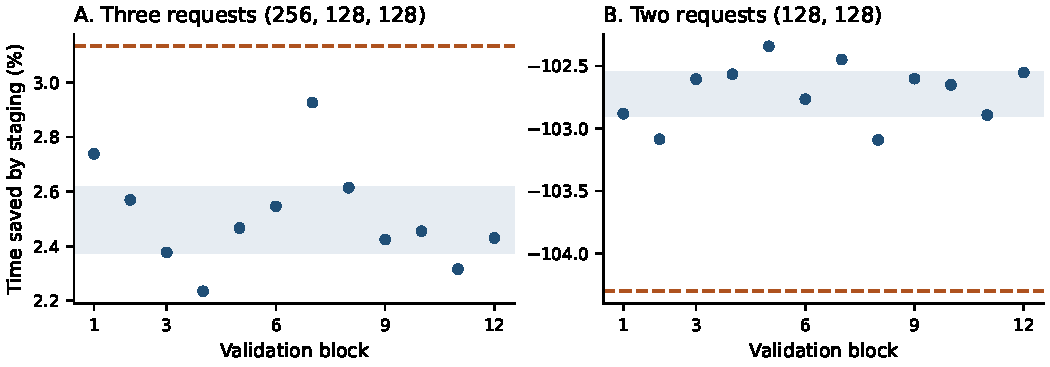
\includegraphics[width=.83\textwidth]{transfer-blocks.pdf}
\caption{Time saved by staging, relative to concurrent admission. Points show the 12 paired wall measurements. The dashed lines give the predictions sealed before validation. Shading spans the third to tenth ordered effects. Each panel uses its own vertical scale. Negative values indicate that waiting increased whole-panel time.}\label{fig:transfer}
\end{figure}

In the three-request test, the arm medians were 1,234 and 1,203 ms. For the two-request control they were 602 and 1,221 ms. Averaging the three-request paired changes allows an additive accounting of the 2.508 percentage points saved. Engine steps returning only cached tokens contributed $+3.165$ points, steps returning a first token contributed $-0.644$, and the remaining host time contributed $-0.013$. Per-step host timing includes engine work beyond kernels. The comparison does not measure waiting time in a multi-tenant queue.

We separately replayed both actions on the first three paths in original order from each of the 200 archived GSM8K questions. The rule was fixed before computing this retrospective analysis. The lengths came from Qwen3-4B-Base, including three paths that reached the 31,744-token cap. Times use the Qwen2.5 three-width clock throughout. Staging helped 66 of 200 panels and increased question-average time by 26.73\% when applied throughout. Even with advance knowledge of the three realized lengths, choosing the faster of these two actions could save only 0.364\% on average (0.205\% by summed times) relative to immediate admission. This calculation concerns three-path prefixes of one archive and exactly two actions. Serving traffic, other actions, and other operating clocks can give different opportunity rates.

\paragraph{What a call guarantee changes.}
In the same archive we also allowed the complete 16-path vote ($N=Q=16$) and checked the full-panel winner of every policy on every question. A synchronous four-sample batch exceeded the serial stopping point by at least two starts on 98 of 200 questions. A four-slot eager scheduler using only the absolute limit did so on 148. Enforcing $B=1$ prevented all such overruns and saved 1.56 starts per question compared with that eager policy, at a 35.36\% increase in question-average modeled time under the DeepSeek 3,968-token clock. A two-sample barrier already respects $B=1$. A deployment needs to value the additional per-question protection enough to justify its latency cost.

\section{Collecting a specified number of verified candidates}\label{app:rpass}
Consider $N$ ordered, irrevocable candidates on the same shared clock. Candidate $i$ reveals a binary verification result after positive work $w_i$. Serial execution stops at its $r$th pass, or at exhaustion of all $N$ candidates, for $1\le r\le N$. Let $K$ denote this stopping index. A policy may start at most $K$ candidates on every compatible completion of its observations. It returns once it observes $r$ passes or completes all $N$. As in voting, work and verifier outcomes are fixed within each comparison.

\begin{proposition}
On any reachable nonterminal history with $s$ observed passes and $f$ failures, the exact cumulative launch frontier is
\[
       \min\{N,s+f+P,r+f\}.
\]
Immediate refill obeys the occupancy comparison \eqref{eq:major} for this task. For fixed slot count $P$, taking the worst case over $N,r$, works and outcomes gives the same exact price ratio $\max_j\widehat c_j/c_j$. The ratio can be attained with finite integer work.
\end{proposition}
\begin{proof}
Initially $J=0\le\min(N,r+f)$, where $J$ is the number launched. Suppose this invariant holds. All observed failures lie in the first $J$ positions. A compatible continuation cannot have stopped before $J$ by the zero-overrun promise on prior starts. From $J$ onward no prefix shorter than $r+f$ can contain $r$ passes. Making all unseen candidates pass attains $\min(N,r+f)$, including when fewer than $r$ passes are possible. The slot cap supplies the other term in the frontier. New failures only increase the cumulative limit. On return with $s=r$, the frontier implies $J\le r+f=s+f\le J$, so all starts have finished. Their indices form the serial stopping prefix by the guarantee. Exhaustion also completes exactly the serial prefix. Thus every admissible schedule performs the same work on a given input.

Greedy's permitted active width $\min(P,N-s-f,r-s)$ cannot increase when more jobs finish. The cumulative frontier is nondecreasing. These properties give the shortened-input comparison and the time compression proof of Appendix~\ref{app:major} with the same jobwise inclusions. The concave-majorant argument then gives the upper ratio.

For sharpness, take a hull chord with endpoints $a<j<b$ attaining the maximum at $j$. Set $r=b$. All candidates fail. Take $a$ long initial jobs of length $L=S/(j-a)$ and $S$ unit jobs where $S=\mathrm{lcm}(b-a,j-a)$. Here $N=a+S\ge b$. With a continuing supply of unit jobs greedy fills to $b$, whereas a policy capped at $j$ fills to $j$. Greedy spends $S/(b-a)$ units of virtual time at width $b$ and the remainder of $L$ at width $a$, counting virtual padding with $c_0=0$ if $a=0$. The comparator spends all $L$ units at width $j$. The time ratio is $\widehat c_j/c_j$. When the maximum is one, a single candidate attains it. No inference about deployed verification policies is required for this corollary.
\end{proof}

\end{document}
